\documentclass{beamer}
\usetheme{Madrid}
\usepackage{pgfplots}
\pgfplotsset{compat=1.15}
\usepackage{mathrsfs}
\usetikzlibrary{arrows}
\usepackage[utf8]{inputenc}
\usepackage{xcolor}
\usepackage{hyperref}
\usepackage{fancyvrb}
\usepackage{comment}
\usepackage{listings}
\usepackage{color}
\definecolor{munsell}{rgb}{0.0, 0.5, 0.69}
\definecolor{dkgreen}{rgb}{0,0.6,0}
\definecolor{gray}{rgb}{0.5,0.5,0.5}
\definecolor{mauve}{rgb}{0.58,0,0.82}
\definecolor{minas}{RGB}{0.244, 0.172, 0.36}
\definecolor{PUJ}{RGB}{44, 86, 151}
\definecolor{PUJ2}{RGB}{43, 93, 156}
\definecolor{PUJ3}{RGB}{20, 52, 107}
\definecolor{cyandk}{rgb}{0.0, 0.72, 0.92}
\setbeamerfont{frametitle}{size=\LARGE ,series=\bfseries}
\setbeamercolor{frametitle}{fg=PUJ2, bg=white} %% title of the beamer
\setbeamercolor{titlelike}
{parent=structure,bg=PUJ2}
\setbeamercolor{title}{fg=white, bg=PUJ3} 
%\setbeamercolor{navigation symbols}{fg=white, bg=white}
\setbeamercolor*{palette primary}{use=structure,fg=black,bg=yellow}
\setbeamercolor*{palette secondary}{use=structure,fg=white,bg=PUJ3}
\setbeamercolor*{palette tertiary}{use=structure,fg=white,bg=PUJ3}

\setbeamercolor{block title}{bg=PUJ3,fg=white}


%% code information
\lstset{frame=tb,
  language=Python,
  aboveskip=3mm,
  belowskip=3mm,
  showstringspaces=false,
  columns=flexible,
  basicstyle={\small\ttfamily},
  numbers=none,
  classoffset=1,
  morekeywords={True,False}, keywordstyle=\color{munsell}, 
  classoffset=0, 
  keywordstyle=\color{blue},  
  commentstyle=\color{dkgreen},
  stringstyle=\color{PUJ3},
  numberstyle=\tiny\color{gray},
  breaklines=true,
  breakatwhitespace=true,
  tabsize=4,
}

%% You can change default language in the middle of document with \lstset{language=Java}.


%% PUT or Remove the logo in a slide.


%% Information topic

\institute{Javeriana}
\date{2020}

\title[Pontificia Universidad Javeriana] %optional
{Introduction to Linear Algebra}
\subtitle{Insights for IA}

\author[Iván Andrés Trujillo Abella] 
{Iván Andrés Trujilllo Abella}

\institute[] 
{
  Facultad de Ingenieria\\
  Pontificia Universidad Javeriana
  \and
  
\textbf{ trujilloiv@javeriana.edu.co}
}

\date[MINTA] % (optional)

\newif\ifplacelogo % create a new conditional
\placelogotrue % set it to true
%\logo{\ifplacelogo\color{red}\rule{.5cm}{.5cm}\fi}
\logo{\ifplacelogo 
\includegraphics[height= 2.0cm]{pujshield.eps}\fi}



\begin{document}



\begin{comment}
\begin{frame}{inner product}
the vectors $\vec{x},\vec{y} \in R^{n}$ the $.$ or inner product is defined as follow:
$\vec{x}= (x_{1},x_{2}, \hdots , x_{n}) $ and $\vec{y_{1}, y_{2}, \hdots , \y_{n}$.
\end{frame}
\end{comment}



\frame{\titlepage}






\begin{frame}{Inner product}
the vectors $\vec{x},\vec{y} \in R^{n}$ the $.$ or inner product is defined as follow:
$\vec{x}= (x_{1},x_{2}, \hdots , x_{n}) $ and $\vec{y} = {y_{1}}, y_{2}, \hdots , y_{n}$.
\begin{equation}
\vec{x}.\vec{y} = \sum_{i=1}^{n} = x_{i}y_{i}
\end{equation}
the sum of each pair of components in each vector is the inner product.
\end{frame}



\begin{frame}{Paralelogram}
\begin{columns}
\column{0.48\textwidth}
\definecolor{uuuuuu}{rgb}{0.26666666666666666,0.26666666666666666,0.26666666666666666}
\begin{tikzpicture}[line cap=round,line join=round,>=triangle 45,scale=0.79]
\begin{axis}[
x=1cm,y=1cm,
axis lines=middle,
xmin=0,
xmax=9,
ymin=0,
ymax=7,
xtick={-1.5,-1,...,12.5},
ytick={-1.5,-1,...,7.5},]
\clip(-1.53295944346379,-1.5357319163741068) rectangle (12.706297059380853,7.615413296841486);
\draw [->,line width=2pt] (0,0) -- (2,4);
\draw [->,line width=2pt] (0,0) -- (6,2);
\draw [->,line width=2pt] (0,0) -- (8,6);
\draw [->,line width=2pt] (2,4) -- (8,6);
\draw [->,line width=2pt] (6,2) -- (8,6);
\begin{scriptsize}
\draw [fill=uuuuuu] (0,0) circle (2pt);
\draw[color=uuuuuu] (0.07920768676665688,0.1836023930335072) node {$A$};
\draw[color=black] (1.0017773162048895,2.1312493885142185) node {$u$};
\draw[color=black] (3.023975392852329,1.1527664482009428) node {$v$};
\draw[color=black] (4.011777218311447,3.147007869410858) node {$w$};
\draw[color=black] (5.018216814062246,5.150568175766614) node {$a$};
\draw[color=black] (6.993820464980482,4.125490809724134) node {$b$};
\end{scriptsize}
\end{axis}
\end{tikzpicture}
\column{0.3\textwidth}
\textit{Parallelogram} in euclidean geometry could be represented by a figure with paralels lines of equal length.
\end{columns}
\end{frame}




\begin{frame}{Unit vector}
the length of a vector or norm $\Vert x \Vert $ it also important and will be defined using 
the pitagoras theorem, as illustrate the following graph.

we can said that a vector $\bar{v}$ is unitary of $ \Vert \bar{v} \Vert = 1$.
think that a vector $y$ is parallel to a $x$ if for instance exist $\lambda$ such that 
$y = \lambda x $. 


to normalize a vector you only need divide by a scalar in this case its longitude thus:
\begin{equation}
\bar{v_{u}} = \frac{\bar{v}}{\Vert  v \Vert} 
\end{equation}
\end{frame}


\begin{frame}{	Cauchy - swartch inequality}
\begin{equation}
\vert \bar{x} . \bar{y} \vert \leq \Vert \bar{x} \Vert \Vert \bar{y} \Vert
\end{equation}

given the angle and inner product $\bar{x}\bar{y} = \Vert \vec{x} \Vert \Vert \vec{y} \Vert cos \theta$ take into account that $\vert\cos \theta \vert \leq 1 , \forall \theta \in \mathbb{R}$
\begin{equation}
\vert \vec{x} . \vec{y} \vert = \vert \Vert \vec{x} \Vert \vert  \vert \Vert \vec{y} \Vert \vert \vert \cos \theta  \vert
\end{equation}
\end{frame} 

\begin{frame}{Projection}
\begin{columns}
\column{0.5\textwidth}
there is a $k$ scalar such that the vectors $\vec{x}, \vec{y}$ be orthogonal. 
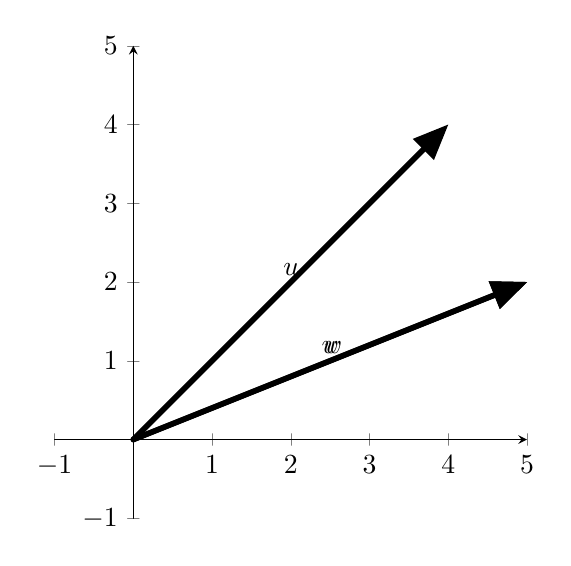
\begin{tikzpicture}[line cap=round,line join=round,>=triangle 45,scale=1]
\begin{axis}[
x=1cm,y=1cm,
axis lines=middle,
xmin=-1,
xmax=5,
ymin=-1,
ymax=5,
xtick={-2,-1,...,13},
ytick={-3,-2,...,7},]
\clip(-2.550209223312352,-3.2608092986131707) rectangle (13.538610513290037,7.051998130462338);
\draw [->,line width=2pt] (0,0) -- (4,4);
\draw [->,line width=2pt] (0,0) -- (5,2);
\draw [->,line width=2pt] (0,0) -- (5,2);
\begin{scriptsize}
\draw[color=black] (2.0075895793543825,2.1528895096235146) node {$u$};
\draw[color=black] (2.52217976675224,1.1657164970643517) node {$v$};
\draw[color=black] (2.52217976675224,1.1657164970643517) node {$w$};
\end{scriptsize}
\end{axis}
\end{tikzpicture}
\column{0.5\textwidth}
Remember that;
\begin{equation}
\cos \theta = \frac{\bar{u}\bar{w}}{\Vert \vec{u} \Vert \Vert \vec{w}\Vert}
\end{equation}
Remember that the project make a parallel line therefore $\cos \theta = \frac{\Vert v_{p} \Vert}{\Vert \vec{u} \Vert}$ where $\vec{W}$ it is the hypohenuse of rectangle.   
\begin{equation}
\Vert \vec{u} \Vert  \cos \theta  = \Vert v_{p} \Vert
\end{equation}
\end{columns}
\end{frame}

\begin{frame}
we calculate the scalar $v_{p}$ now we are interested in the vector, therefore:
\begin{equation}
\frac{\vec{w}}{\Vert W \Vert} V_{p} = \vec{V_{p}}
\end{equation}
Notice that $\vec{v_{p}}$ refer to the vector while in other case $\vec{v_{p}}$ refer to the magnitude.
\begin{equation}
\vec{v_{p}} = \frac{\vec{u}\vec{w}}{\Vert \vec{w} \Vert } \vec{w}
\end{equation}
\end{frame}









\end{document}